%% sheaf_cohomology_actp.tex
%% arXiv submission draft — cs.CR / cs.MA
%% Authors: Justin Roosch\"{u}z, Damir Mujić
%% AGIRAILS Inc.
%%
%% Build: pdflatex sheaf_cohomology_actp.tex  (twice for cross-refs)
%%

\documentclass[11pt]{article}

%% ─── Core maths ───────────────────────────────────────────────────────────────
\usepackage{amsmath,amssymb,amsthm}
\usepackage{mathtools}

%% ─── Theorem environments ─────────────────────────────────────────────────────
\theoremstyle{plain}
\newtheorem{theorem}{Theorem}[section]
\newtheorem{proposition}[theorem]{Proposition}
\newtheorem{lemma}[theorem]{Lemma}
\newtheorem{corollary}[theorem]{Corollary}

\theoremstyle{definition}
\newtheorem{definition}[theorem]{Definition}
\newtheorem{example}[theorem]{Example}
\newtheorem{remark}[theorem]{Remark}

%% ─── Tables and figures ───────────────────────────────────────────────────────
\usepackage{booktabs}
\usepackage{array}
\usepackage{multirow}
\usepackage{xcolor}
\usepackage{graphicx}

%% ─── Code listings ────────────────────────────────────────────────────────────
\usepackage{listings}
\lstset{
  basicstyle=\small\ttfamily,
  keywordstyle=\bfseries\color{blue!70!black},
  commentstyle=\itshape\color{gray},
  stringstyle=\color{green!50!black},
  backgroundcolor=\color{gray!8},
  frame=single,
  rulecolor=\color{gray!40},
  numbers=left,
  numberstyle=\tiny\color{gray},
  numbersep=6pt,
  breaklines=true,
  captionpos=b
}

%% ─── Algorithms ───────────────────────────────────────────────────────────────
\usepackage[ruled,vlined,linesnumbered]{algorithm2e}

%% ─── TikZ for diagrams ────────────────────────────────────────────────────────
\usepackage{tikz}
\usepackage{tikz-cd}
\usetikzlibrary{arrows.meta, positioning, shapes.geometric, fit, calc}

%% ─── Layout ───────────────────────────────────────────────────────────────────
\usepackage[margin=1.1in]{geometry}
\usepackage{microtype}
\usepackage{parskip}
\usepackage{abstract}
\setlength{\parindent}{0pt}
\setlength{\parskip}{6pt plus 2pt minus 1pt}
\setlength{\absleftindent}{0pt}
\setlength{\absrightindent}{0pt}
\setlength{\absparsep}{6pt plus 2pt minus 1pt}

% Tectonic/XeTeX may request TU/lmr/bx/sc for run-in paragraph heads.
% Declare an explicit fallback at begin-document time, after font setup.
\AtBeginDocument{%
  \makeatletter
  \DeclareFontShape{TU}{lmr}{bx}{sc}{<->ssub*lmr/bx/n}{}
  \makeatother
}

%% ─── Hyperlinks ───────────────────────────────────────────────────────────────
\usepackage[colorlinks=true,
            linkcolor=blue!60!black,
            citecolor=green!40!black,
            urlcolor=blue!70!black,
            pdftitle={Sheaf Cohomology for Settlement Protocol Verification},
            pdfauthor={Roosch\"{u}z, Mujić -- AGIRAILS Inc.}]{hyperref}

%% ─── Macros ───────────────────────────────────────────────────────────────────
\newcommand{\Fsh}{\mathcal{F}}         % sheaf
\newcommand{\Gsh}{\mathcal{G}}         % second sheaf
\newcommand{\Czero}{C^{0}}
\newcommand{\Cone}{C^{1}}
\newcommand{\Ctwo}{C^{2}}
\newcommand{\Hzero}{H^{0}}
\newcommand{\Hone}{H^{1}}
\newcommand{\Htwo}{H^{2}}
\newcommand{\deltazero}{\delta_{0}}
\newcommand{\deltaone}{\delta_{1}}
\newcommand{\stalk}[1]{\Fsh(#1)}
\newcommand{\RR}{\mathbb{R}}
\newcommand{\ZZ}{\mathbb{Z}}
\newcommand{\rank}{\operatorname{rank}}
\newcommand{\im}{\operatorname{im}}
\newcommand{\kers}{\operatorname{ker}}
\newcommand{\dimn}{\operatorname{dim}}

% Filename in monospace that allows line-breaks after each underscore.
% Use this for long underscored filenames in body prose (not in headings/captions).
\newcommand{\codefile}[1]{\texttt{#1}}

% State names
\newcommand{\sINIT}{\textsc{Initiated}}
\newcommand{\sQUOT}{\textsc{Quoted}}
\newcommand{\sCOMM}{\textsc{Committed}}
\newcommand{\sINPROG}{\textsc{InProgress}}
\newcommand{\sDELIV}{\textsc{Delivered}}
\newcommand{\sSETTL}{\textsc{Settled}}
\newcommand{\sDISP}{\textsc{Disputed}}
\newcommand{\sCANC}{\textsc{Cancelled}}

%% ─── Document ─────────────────────────────────────────────────────────────────
\begin{document}

\title{\textbf{Sheaf Cohomology for Settlement Protocol Verification}\\[4pt]
       \large Measuring Topological Completeness and Information Asymmetry in ACTP}

\author{
  Justin Roosch\"{u}z\thanks{justin@agirails.io}
  \and Damir~Mujić\thanks{damir@agirails.io}
}

\date{%
  AGIRAILS Inc. \\[4pt]
  \small \today
}

\maketitle

\begin{abstract}
Autonomous AI agents are non-deterministic: they can refuse to deliver, refuse
to pay, or interpret the same task differently each time.  This makes
agent-to-agent commerce structurally risky, and the classical answer is
escrow --- a neutral party that holds funds until both sides perform.  For
autonomous agents, that neutral party is a smart contract.  But this only
relocates the problem.  The escrow protocol itself must be provably correct,
and ``provably correct'' is not one thing.

This paper asks a specific part of that question: when an agent settlement
protocol exposes local state at each step, does that state assemble into a
globally consistent picture, and if not, where does it fail?  We answer with
cellular sheaf cohomology.  Two sheaves are constructed over the 8-state
lifecycle of ACTP, the Agent Commerce Transaction Protocol.  A state-based
sheaf measures structural completeness: whether local state globalises.  A
participant-based sheaf measures information asymmetry: whether all parties
can see what they need to verify the outcome.

On the state sheaf, $\Hone = 24$ when the protocol is treated as a bare
graph and $\Hone = 0$ once 2-cells encoding its parallel paths are added.
The protocol is topologically complete: every piece of local state carries
through every transition into a single consistent global view.  On the
participant sheaf, under a conservative semantic model, $\Hone$ stays between
6 and 8 at every protocol state.  That gap is not an error.  It is the
information that still needs to be exchanged off-chain or via an oracle for
all parties to agree --- and quantifying it is part of the contribution.
A separate exact six-channel raw-visibility supplement yields $\Hone = 0$ at
every state after public-face completion, so the conservative semantic
values are best read as an upper-bound diagnostic rather than an exact
raw-visibility invariant.

Structural completeness is necessary but not sufficient for trustlessness.
The two sheaves answer orthogonal questions and are meant to be read
together.  We also provide open-source tooling: a YAML-driven $\Hone$ linter
with CI integration; 1-complex rank computations cross-validated using exact
rational arithmetic; and a participant visibility model checked against the
live ACTP SDK as of 2026.  To our knowledge this is the first application
of sheaf cohomology to smart contract escrow protocol verification, building
on Felber et al.'s task-sheaf framework but extending it with a participant
information-asymmetry sheaf.
\end{abstract}

\clearpage
\tableofcontents

\clearpage

%% ═══════════════════════════════════════════════════════════════════════════════
\section{Introduction}
\label{sec:intro}
%% ═══════════════════════════════════════════════════════════════════════════════

Autonomous AI agents are non-deterministic.  Given the same task twice, an
agent may produce different outputs, take different paths to reach them, or
decide not to proceed at all.  This is not a deficiency.  It is a consequence
of the decision-making capacity that makes agents useful in the first place.
A deterministic agent is a program.  A non-deterministic agent is an entity
that chooses.

But non-determinism makes economic interaction between agents structurally
risky.  An agent that receives payment before delivering may not deliver.
An agent that delivers before being paid may not get paid.  The same pattern
exists in human commerce, and it is why escrow exists: a neutral third party
holds funds until both sides perform.  For autonomous agents, that neutral
third party is a smart contract.

This does not eliminate the problem.  It relocates it.  A smart contract is
only as trustworthy as its design, and ``trustworthy'' needs to mean
something specific when the contract is supposed to enforce guarantees no
human is watching.  A bug in the escrow logic, a missing state transition,
an asymmetry in what each party can observe at a critical moment --- any of
these can break the guarantee that the escrow was supposed to provide.

So the question becomes: how do you prove that an escrow protocol actually
holds together?  Not test it.  Not audit the code line by line.  \emph{Prove}
it, in the sense that a structural property of the protocol --- independent
of any particular execution or any particular auditor --- can be formally
verified and independently reproduced.

\paragraph{What existing tools answer, and what they miss.}
Model checkers like TLA$^+$~\cite{Lamport2002} and Alloy~\cite{Jackson2012}
verify temporal and relational properties by enumerating reachable states and
checking that safety and liveness invariants hold across traces.  They are
powerful, but they treat all data as undifferentiated.  They cannot
distinguish a missing \emph{dimension} of shared state from a missing
\emph{transition}.  Smart-contract auditors like
Certora~\cite{Certora2026}, Echidna~\cite{Echidna2020}, and
Slither~\cite{Slither2019} check code-level safety: reentrancy, overflow,
access control.  They
operate one level below the protocol, on the Solidity implementation rather
than the state machine the implementation is meant to realise.  Both layers
are necessary, and neither addresses the question we want to answer: does the
information the protocol exposes at each step actually assemble into a
globally consistent picture, and if not, where does it fail?

\paragraph{Sheaf cohomology as the framework.}
This is the question cellular sheaf cohomology was designed to answer.  A
cellular sheaf assigns a vector space --- the \emph{stalk} --- to each cell of
a cell complex, and equips adjacent cells with \emph{restriction maps}
encoding how data flows across boundaries.  The first cohomology group
$\Hone$ counts the independent obstructions to globalising locally consistent
data.  $\Hone = 0$ means every assignment of local data that agrees on shared
dimensions can be assembled into a globally consistent section.  $\Hone \neq
0$ gives a precise, computable count of the dimensions that prevent this.

Applied to a settlement protocol, this yields two complementary measurements.
A \emph{state-based sheaf} places stalks on protocol states (their observable
data dimensions) and on transitions (the fields that must agree across them);
its $\Hone$ measures structural completeness --- whether local state at each
step assembles into a consistent global view.  A \emph{participant-based
sheaf} places stalks on the protocol's principals (requester, provider,
escrow vault, kernel) and on the information channels between them; its
$\Hone$ measures information asymmetry --- whether any dimension of protocol
state is accessible to some principals but hidden from others.

The two sheaves answer orthogonal questions.  A protocol can be structurally
complete yet participant-asymmetric, with one party unable to verify what
another knows.  Trustlessness in a strict sense requires both, and the
participant sheaf further admits two natural resolutions: a conservative
\emph{semantic} model that treats off-chain evidence as opaque, and an exact
\emph{raw-visibility} model that credits public on-chain observability
through public view functions.  The gap between these two models formalises
the difference between what participants can \emph{see} and what they can
\emph{verify}.

\paragraph{Application: ACTP.}
The application in this paper is the Agent Commerce Transaction Protocol
(ACTP)~\cite{AGIRAILSsdk}, an 8-state escrow lifecycle for autonomous agents
running on Base.  ACTP handles request, quote, commitment, in-progress work,
delivery, and settlement, with side branches for disputes and cancellations.
The protocol targets Base mainnet deployment, and at least one end-to-end
settlement transaction has been observed on Base mainnet
~\cite{ACTPmainnettx}.  The implementation we analyse
is \texttt{sdk-js} package version \texttt{3.2.0} (commit \texttt{d5dc886})
and the corresponding \texttt{actp-kernel} commit \texttt{91f4f90}.

\paragraph{Scope of formal claims.}
Unless explicitly marked otherwise, every theorem and rank computation in
Sections~\ref{sec:state_sheaf} through~\ref{sec:participant} is a statement
about a reduced supplementary artifact --- a YAML protocol specification
labelled ``ACTP v2.7'' --- and, for 2-complex claims, about an explicit
10-face refinement declared in Appendix~\ref{app:faces}.  Code inspection and
the mainnet transaction trace are included as implementation evidence.  They
are not premises in the cohomology proofs.  This distinction matters because
the paper's mathematical claims are about a model, and the model's fidelity
to the deployed protocol is a separate, empirical question that we address
but do not conflate with the proofs.

\paragraph{Related work.}
Felber et al.~\cite{Felber2025} recently applied cellular sheaves to
distributed task solvability, showing that sheaf cohomology encodes
obstructions to finding valid protocol solutions.  Their framework treats
distributed computing tasks in general; ours addresses a specific class of
them --- settlement protocols --- and adds participant information asymmetry
as a second construction.  Background on cellular sheaves is drawn from
Ghrist~\cite{Ghrist2014} and Curry~\cite{Curry2014}; the spectral theory of
Hansen and Ghrist~\cite{HansenGhrist2019} provides the algebraic foundation.
Robinson~\cite{Robinson2014} situates sheaf theory within signal processing
on networks, which informs our restriction-map construction.

\paragraph{Paper roadmap.}
Section~\ref{sec:background} reviews cellular sheaves and ACTP.
Section~\ref{sec:state_sheaf} constructs the state-based sheaf and derives
$\Hone$ for the 1-complex and 2-complex.
Section~\ref{sec:evolution} analyses the dispute process and the attestation
layer.
Section~\ref{sec:participant} presents the participant-based sheaf.
Section~\ref{sec:tooling} describes the current supplementary tooling.
Section~\ref{sec:related} situates the work.
Section~\ref{sec:discussion} discusses limitations and future work.
Section~\ref{sec:conclusion} concludes.

%% ═══════════════════════════════════════════════════════════════════════════════
\section{Background}
\label{sec:background}
%% ═══════════════════════════════════════════════════════════════════════════════

\subsection{Cellular Sheaves}
\label{sec:sheaves}

Before the formalism, a one-line intuition.  A cellular sheaf is a way to
attach local data to the pieces of a space (vertices, edges, faces) and ask:
do all the local pieces fit together into a consistent global picture?  When
they do, the sheaf has a global section.  When they do not, the obstruction
is counted by cohomology.  This section makes that precise.

Let $X$ be a regular cell complex.  Write $X^{(k)}$ for the set of
$k$-cells and $\sigma \leq \tau$ when cell $\sigma$ is a face of cell
$\tau$.

\begin{definition}[Cellular sheaf]\label{def:sheaf}
A cellular sheaf $\Fsh$ on $X$ over $\RR$ consists of
\begin{enumerate}
  \item a finite-dimensional $\RR$-vector space $\Fsh(\sigma)$ for each cell
        $\sigma \in X$, and
  \item for each face relation $\sigma \le \tau$, a linear map
  \[
    \rho_{\sigma\to\tau} \colon \Fsh(\sigma) \to \Fsh(\tau),
  \]
  subject to functoriality: if $\sigma \le \tau \le \upsilon$ then
  $\rho_{\sigma\to\upsilon} = \rho_{\tau\to\upsilon}\circ \rho_{\sigma\to\tau}$.
\end{enumerate}
\end{definition}

\paragraph{Cochain complex.}
Given $\Fsh$ on a cell complex with 0-cells (vertices) $V$, 1-cells (edges)
$E$, and 2-cells (faces) $F$, orient each edge $e = (u,v)$ with tail
$t(e) = u$ and head $h(e) = v$, and orient each face $f$ with an ordered
boundary $\partial f$.  Define
\[
  \Czero = \bigoplus_{v \in V} \Fsh(v), \quad
  \Cone  = \bigoplus_{e \in E} \Fsh(e), \quad
  \Ctwo  = \bigoplus_{f \in F} \Fsh(f).
\]
The \textbf{coboundary maps} are:
\begin{align}
  (\deltazero \xi)(e) &= \rho_{h(e)\to e}\bigl(\xi(h(e))\bigr)
                       - \rho_{t(e)\to e}\bigl(\xi(t(e))\bigr),
                       \label{eq:delta0} \\
  (\deltaone \eta)(f) &= \sum_{e \in \partial f} \epsilon(e,f)\,
                         \rho_{e\to f}\bigl(\eta(e)\bigr),
                       \label{eq:delta1}
\end{align}
where $\epsilon(e,f) \in \{+1,-1\}$ is the incidence sign.

\begin{definition}[Sheaf cohomology]\label{def:cohomology}
The cohomology groups of $\Fsh$ are
\[
  \Hzero(\Fsh) = \ker(\deltazero), \quad
  \Hone(\Fsh)  = \frac{\ker(\deltaone)}{\im(\deltazero)}, \quad
  \Htwo(\Fsh)  = \frac{\Ctwo}{\im(\deltaone)}.
\]
\end{definition}

\begin{remark}
$\Hzero(\Fsh)$ is the space of \emph{global sections}: assignments of
vectors to vertices that are consistent across every edge.  Think of it as
the set of ways the local data can be stitched together without tearing.
$\Hone(\Fsh)$ counts the independent obstructions to stitching:
$\dimn \Hone = \dimn \ker(\deltaone) - \rank(\deltazero)$.  For a 1-complex
(no 2-cells), $\ker(\deltaone) = \Cone$ so
$\dimn \Hone = \dimn \Cone - \rank(\deltazero)$, which can overcount when
cycles carry redundant information.  Adding 2-cells reduces $\Hone$ by
$\rank(\deltaone)$.  Put differently: $\Hone = 0$ means every locally
consistent assignment extends to a global one; $\Hone > 0$ means some do
not, and the number tells you how many dimensions of disagreement exist.
\end{remark}

\subsection{The Agent Commerce Transaction Protocol (ACTP)}
\label{sec:actp}

Before the formal description, a concrete scenario.  A requester agent needs
a document translated and posts a task with a deadline.  A provider agent
responds with a price.  The requester accepts, and USDC is locked in escrow
on-chain.  The provider does the work and marks it delivered.  If the
requester accepts the result, the funds release to the provider.  If not,
either side can open a dispute inside a fixed window, and resolution follows
a privileged path. This is ACTP.

Formally, ACTP is the settlement layer of the AGIRAILS
infrastructure~\cite{AGIRAILSsdk}.  It defines a payment lifecycle in which an
AI agent (\emph{Requester}) purchases a service from another agent
(\emph{Provider}) via a non-custodial on-chain USDC escrow enforced by the
\emph{ACTPKernel} smart contract.

\paragraph{States.}
ACTP defines eight protocol states:
\[
  \sINIT \to \sQUOT \to \sCOMM \to \sINPROG \to \sDELIV \to \sSETTL,
\]
with side-branches to $\sDISP$ (dispute) and $\sCANC$ (cancellation).
Table~\ref{tab:states} lists each state and the primary data dimensions
observable at that state.

\begin{table}[h]
\centering
\caption{ACTP v2.7 reduced observable basis used by the current supplementary artifact.}
\label{tab:states}
\small
\begin{tabular}{@{}lcp{7.5cm}@{}}
\toprule
\textbf{State} & \textbf{Dim} & \textbf{Observable dimensions (stalk basis)} \\
\midrule
\sINIT    & 6 & transaction\_id, requester\_address, provider\_address, amount, deadline, service\_hash \\
\sQUOT   & 7 & + quote\_details \\
\sCOMM   & 8 & + escrow\_id, escrow\_balance \\
\sINPROG & 9 & + work\_started\_at \\
\sDELIV  & 11 & + delivery\_proof, dispute\_window\_end \\
\sSETTL  & 9 & transaction\_id, requester\_address, provider\_address, amount, service\_hash, escrow\_id, settlement\_tx, provider\_payout, platform\_fee \\
\sDISP   & 10 & transaction\_id, requester\_address, provider\_address, amount, deadline, service\_hash, escrow\_id, escrow\_balance, delivery\_proof, dispute\_reason \\
\sCANC   & 6  & transaction\_id, requester\_address, provider\_address, amount, cancellation\_reason, refund\_tx \\
\bottomrule
\end{tabular}
\end{table}

\begin{remark}[Semantic observables vs.\ raw storage]
The stalk basis in Table~\ref{tab:states} is a basis of \emph{semantic
observables}, not a one-to-one copy of raw Solidity storage slots.  Depending
on the dimension, an observable may be assembled from contract storage,
events, calldata, SDK-managed payloads, or public off-chain artifacts.  This
distinction matters for participant visibility: public hashes or references
are not equivalent to full semantic content.
\end{remark}

\paragraph{Transitions.}
The 12 directed transitions of the current reduced-basis ACTP v2.7 supplementary artifact are:

\begin{enumerate}
  \item $\sINIT \xrightarrow{e_1} \sQUOT$: provider submits quote
  \item $\sINIT \xrightarrow{e_2} \sCOMM$: requester links funded escrow directly
  \item $\sINIT \xrightarrow{e_3} \sCANC$: requester cancels before quote
  \item $\sQUOT \xrightarrow{e_4} \sCOMM$: requester accepts quote and links escrow
  \item $\sQUOT \xrightarrow{e_5} \sCANC$: quote expires or is rejected
  \item $\sCOMM \xrightarrow{e_6} \sINPROG$: provider begins execution
  \item $\sCOMM \xrightarrow{e_7} \sCANC$: post-commit cancellation / refund path
  \item $\sINPROG \xrightarrow{e_8} \sDELIV$: provider marks delivery
  \item $\sINPROG \xrightarrow{e_9} \sCANC$: execution abort / refund path
  \item $\sDELIV \xrightarrow{e_{10}} \sSETTL$: requester confirms, or anyone settles after the dispute window
  \item $\sDELIV \xrightarrow{e_{11}} \sDISP$: requester or provider opens dispute within the dispute window
  \item $\sDISP \xrightarrow{e_{12}} \sSETTL$: privileged dispute resolution
\end{enumerate}

The live contract additionally permits a privileged $\sDISP \to \sCANC$
resolution edge.  The current open-source state-sheaf artifact omits that
administrative refund edge, so the numerical state-based results in this paper
apply to the 12-edge artifact above unless stated otherwise.

\paragraph{Parallel paths and cycles.}
ACTP has three structurally significant parallel paths:
\begin{itemize}
  \item \emph{Direct happy path:} $\sINIT \to \sCOMM \to \sINPROG
        \to \sDELIV \to \sSETTL$ (4 transitions).
  \item \emph{Quoted happy path:} $\sINIT \to \sQUOT \to \sCOMM \to
        \sINPROG \to \sDELIV \to \sSETTL$ (5 transitions).
  \item \emph{Dispute path:} $\sDELIV \to \sDISP \to \sSETTL$ in parallel
        with $\sDELIV \to \sSETTL$ (creates a cycle / face).
\end{itemize}
Four cancellation branches from $\sINIT$, $\sQUOT$, $\sCOMM$, $\sINPROG$
each form short paths to $\sCANC$.  In the current public 2-complex artifact,
these parallel paths are encoded explicitly as faces in the YAML supplement,
while the same linter can still be run on the underlying 1-complex alone.

Figure~\ref{fig:state_machine} depicts the ACTP state machine.

\begin{figure}[h]
\centering
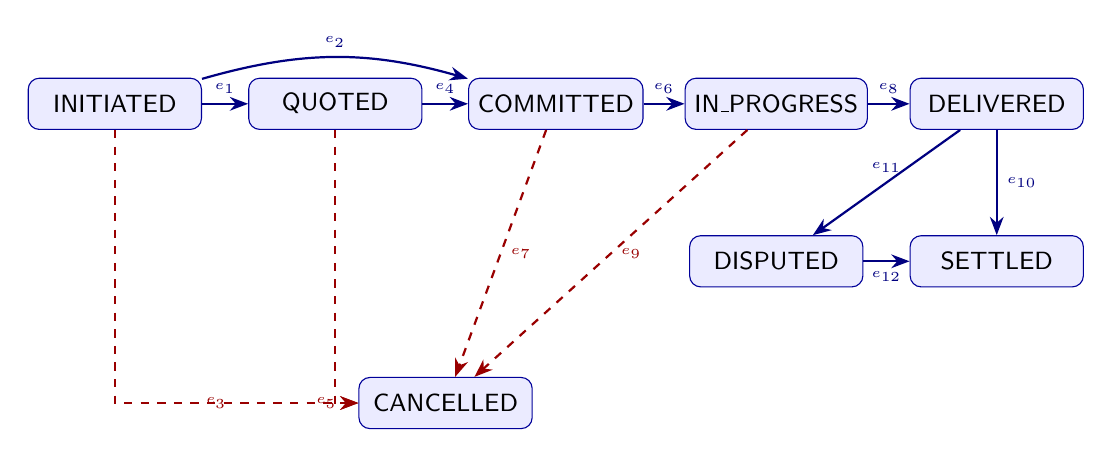
\begin{tikzpicture}[
  state/.style={rectangle, rounded corners=4pt, draw=blue!60!black,
                fill=blue!8, minimum width=2.2cm, minimum height=0.65cm,
                font=\small\sffamily},
  trans/.style={-Stealth, thick, blue!50!black},
  ctrans/.style={-Stealth, thick, red!60!black, dashed},
  every node/.style={font=\small}
]
% Main happy path — left to right
\node[state] (init)    at (0,0)      {INITIATED};
\node[state] (quot)    at (2.8,0)    {QUOTED};
\node[state] (comm)    at (5.6,0)    {COMMITTED};
\node[state] (inprog)  at (8.4,0)    {IN\_PROGRESS};
\node[state] (deliv)   at (11.2,0)   {DELIVERED};
\node[state] (settl)   at (11.2,-2)  {SETTLED};
\node[state] (disp)    at (8.4,-2)   {DISPUTED};
\node[state] (canc)    at (4.2,-3.8) {CANCELLED};

% Happy path transitions
\draw[trans] (init)   -- node[above,font=\tiny]{$e_1$} (quot);
\draw[trans] (init)   to[bend left=16] node[above,font=\tiny]{$e_2$} (comm);
\draw[trans] (quot)   -- node[above,font=\tiny]{$e_4$} (comm);
\draw[trans] (comm)   -- node[above,font=\tiny]{$e_6$} (inprog);
\draw[trans] (inprog) -- node[above,font=\tiny]{$e_8$} (deliv);
\draw[trans] (deliv)  -- node[right,font=\tiny]{$e_{10}$} (settl);

% Dispute cycle
\draw[trans] (deliv)  -- node[above,font=\tiny]{$e_{11}$} (disp);
\draw[trans] (disp)   -- node[below,font=\tiny]{$e_{12}$} (settl);

% Cancellation branches
\draw[ctrans] (init)   |- node[near end, left,font=\tiny]{$e_3$}  (canc);
\draw[ctrans] (quot)   |- node[near end, left,font=\tiny]{$e_5$}  (canc);
\draw[ctrans] (comm)   -- node[right,font=\tiny]{$e_7$}            (canc);
\draw[ctrans] (inprog) -- node[right,font=\tiny]{$e_9$}            (canc);
\end{tikzpicture}
\caption{ACTP v2.7 state machine for the 12-edge supplementary artifact.
         Blue solid arrows = nominal path; red dashed arrows = cancellation.
         The live contract additionally exposes a privileged
         $\sDISP \to \sCANC$ resolution edge not drawn here.}
\label{fig:state_machine}
\end{figure}

%% ═══════════════════════════════════════════════════════════════════════════════
\section{State-Based Sheaf Construction}
\label{sec:state_sheaf}
%% ═══════════════════════════════════════════════════════════════════════════════

\subsection{Vertex and Edge Stalks}
\label{sec:stalks}

The state-based sheaf $\Fsh_S$ attaches a vector space to every protocol
state and every transition between states.

\begin{definition}[State stalk]\label{def:state_stalk}
The stalk $\Fsh_S(v)$ at state $v$ is $\RR^d$ where $d = \dimn(v)$ is the
number of named data fields observable at that state (Table~\ref{tab:states}).
\end{definition}

\begin{definition}[Transition stalk]\label{def:trans_stalk}
For transition $e = (u, v)$, the stalk $\Fsh_S(e) = \RR^s$ where $s$ is
the number of fields \emph{shared} between $u$ and $v$ --- i.e., fields that
must agree across the transition.
\end{definition}

\begin{definition}[Restriction maps]\label{def:restriction}
For an edge $e = (u,v)$:
\begin{itemize}
  \item $\rho_{u\to e} \colon \Fsh_S(u) \to \Fsh_S(e)$: projection onto
        the shared fields.
  \item $\rho_{v\to e} \colon \Fsh_S(v) \to \Fsh_S(e)$: projection onto
        the shared fields.
\end{itemize}
\end{definition}

The coboundary $\deltazero$ is therefore (from~\eqref{eq:delta0}):
\[
  (\deltazero\xi)(e) = \rho_{v\to e}(\xi(v)) - \rho_{u\to e}(\xi(u)),
\]
which is zero precisely when the data at $u$ and $v$ agree on all shared
dimensions.

Figure~\ref{fig:sheaf_example} illustrates the construction on a single ACTP
transition, $e_1 \colon \sINIT \to \sQUOT$.

\begin{figure}[h]
\centering
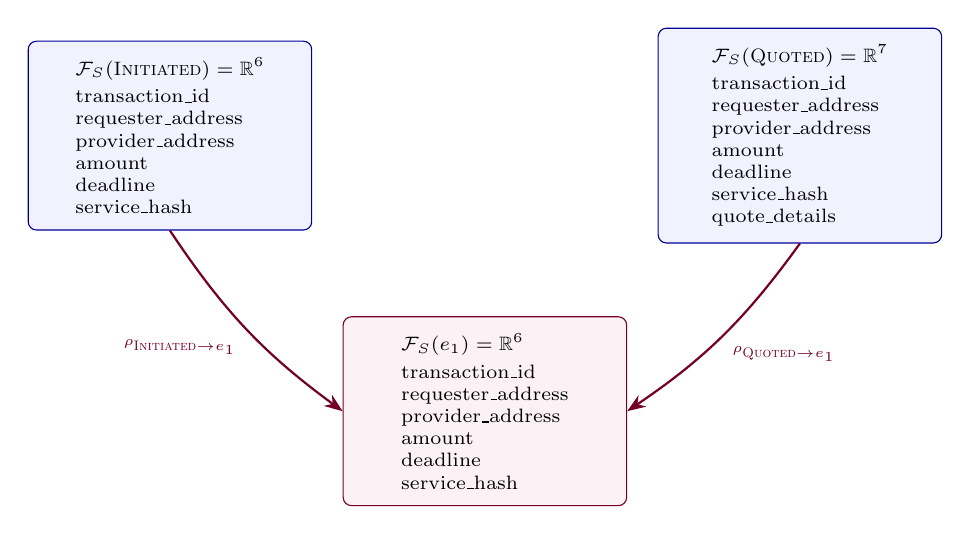
\begin{tikzpicture}[
  stalk/.style={rectangle, rounded corners=3pt, draw=blue!60!black,
                fill=blue!5, minimum width=3.6cm, align=left,
                inner sep=6pt, font=\scriptsize},
  edgestalk/.style={rectangle, rounded corners=3pt, draw=purple!60!black,
                    fill=purple!5, minimum width=3.6cm, align=left,
                    inner sep=6pt, font=\scriptsize},
  arrow/.style={-Stealth, thick, purple!60!black},
  every node/.style={font=\small}
]

% Vertex stalks
\node[stalk] (init) at (0,0) {%
  $\Fsh_S(\sINIT) = \RR^{6}$ \\[2pt]
  transaction\_id \\
  requester\_address \\
  provider\_address \\
  amount \\
  deadline \\
  service\_hash
};

\node[stalk] (quot) at (8,0) {%
  $\Fsh_S(\sQUOT) = \RR^{7}$ \\[2pt]
  transaction\_id \\
  requester\_address \\
  provider\_address \\
  amount \\
  deadline \\
  service\_hash \\
  quote\_details
};

% Edge stalk
\node[edgestalk] (edge) at (4,-3.5) {%
  $\Fsh_S(e_1) = \RR^{6}$ \\[2pt]
  transaction\_id \\
  requester\_address \\
  provider\_address \\
  amount \\
  deadline \\
  service\_hash
};

% Restriction map arrows
\draw[arrow] (init.south) to[bend right=10]
  node[midway, below left, font=\tiny]{$\rho_{\sINIT \to e_1}$} (edge.west);
\draw[arrow] (quot.south) to[bend left=10]
  node[midway, below right, font=\tiny]{$\rho_{\sQUOT \to e_1}$} (edge.east);

\end{tikzpicture}
\caption{The state-based sheaf over the transition
$e_1 \colon \sINIT \to \sQUOT$.  Each vertex stalk is a real vector space
whose basis is the observable fields at that state.  The edge stalk is the
subspace spanned by the fields shared between the two endpoints: all six
INITIATED fields carry through to QUOTED.  The restriction maps are
orthogonal projections of each vertex stalk onto the edge stalk.  The
coboundary $\deltazero\xi(e_1)$ is zero precisely when the restrictions from
the two endpoints agree.  Here the only field in QUOTED without a
counterpart in INITIATED is \texttt{quote\_details}, which is added by the
transition and has no corresponding component in $\Fsh_S(e_1)$.}
\label{fig:sheaf_example}
\end{figure}

\subsection{Coboundary Matrices}
\label{sec:matrices}

Let $n_v = \sum_{v} \dimn(v)$ and $n_e = \sum_{e} \dimn(e)$.  For the
current reduced-basis ACTP v2.7 supplementary artifact:
\begin{align*}
  \dimn(\Czero) &= 6 + 7 + 8 + 9 + 11 + 9 + 10 + 6 = 66, \\
  \dimn(\Cone)  &= \sum_{i=1}^{12} s(e_i)
\end{align*}
where $s(e_i)$ is the shared-field count for each transition.  After
computing shared dimensions for each of the 12 transitions (e.g.,
$s(e_1) = 6$ for $\sINIT \to \sQUOT$, $s(e_{10}) = 6$ for $\sDELIV \to
\sSETTL$), we obtain $\dimn(\Cone) = 72$.

\begin{remark}
The current YAML-driven engine encodes each state's \texttt{stalks} and
derives edge overlap by field intersection.  It programmatically assembles
$\deltazero$ and, when a \texttt{faces:} section is present, also assembles
$\deltaone$.  Running \texttt{python3 h1\_lint.py --2complex} on the public
supplement reproduces the 2-complex results reported below.
\end{remark}

The matrix $\deltazero \in \RR^{72 \times 66}$ has rank computed via
NumPy \texttt{linalg.matrix\_rank} with tolerance $10^{-9}$.  All rank
computations for $\deltazero$ (the 1-complex results) have been
cross-validated using exact rational arithmetic (Python
\texttt{fractions} module, see supplementary \texttt{verify\_rational.py});
results agree with the floating-point computation in every reported case.

\subsection{Results: 1-Complex}
\label{sec:results_1complex}

Table~\ref{tab:h1_1complex} summarises $\Hone$ for several subgraphs of
ACTP v2.7, treating the protocol as a 1-complex (no 2-cells).

\begin{table}[h]
\centering
\caption{$\Hone$ on the 1-complex for ACTP v2.7 subgraphs in the current supplementary artifact.}
\label{tab:h1_1complex}
\resizebox{\textwidth}{!}{%
\begin{tabular}{@{}lrrrrl@{}}
\toprule
\textbf{Subgraph} & $\dimn\Czero$ & $\dimn\Cone$ & $\rank(\deltazero)$ & $\dimn\Hone$ & \textbf{Interpretation} \\
\midrule
Full protocol              & 66 & 72 & 48 & 24 & Aggregate obstruction count \\
Direct happy path          & 43 & 29 & 29 &  0 & Direct funded path is consistent \\
Quoted linear path         & 50 & 35 & 35 &  0 & Quoted route alone is consistent \\
Quote/commit comparison    & 50 & 41 & 35 &  6 & Quote-specific data not preserved across both commit routes \\
Dispute path               & 30 & 21 & 15 &  6 & Dispute subgraph asymmetry \\
Cancellation subgraph      & 36 & 42 & 24 & 18 & Terminal-state field loss dominates \\
\bottomrule
\end{tabular}
}
\end{table}

\paragraph{Interpretation.}
The 18 cancellation obstructions arise because the four cancellation
branches from $\sINIT$, $\sQUOT$, $\sCOMM$, and $\sINPROG$ each arrive at
$\sCANC$ carrying only the basic transactional core
(\texttt{transaction\_id}, \texttt{requester\_address},
\texttt{provider\_address}, \texttt{amount}), leaving terminal-state fields
unmatched.  The 6 dispute obstructions reflect that $\sDISP$ and $\sSETTL$
do not share all fields that the direct $\sDELIV \to \sSETTL$ path would
carry.  The additional 6 obstructions do not arise on the quoted linear path
by itself.  They arise when the direct route $\sINIT \to \sCOMM$ is compared
with the quoted route $\sINIT \to \sQUOT \to \sCOMM$ inside the same
1-complex subgraph.

\subsection{2-Cell Extension}
\label{sec:2cell}

The 1-complex count of 24 is an artefact: it treats parallel paths as
independent rather than recognising them as boundaries of 2-cells.

\begin{definition}[Face / 2-cell]\label{def:face}
A \emph{face} of the state graph is specified by two directed paths
$p^{+}$ and $p^{-}$ with the same source and target.  Its boundary is the
formal difference
\[
  \partial f = p^{+} - p^{-},
\]
and the face stalk $\Fsh_S(f)$ is the intersection of all edge stalks that
appear on $\partial f$.
\end{definition}

\begin{remark}
This convention selects the maximal face stalk compatible with the restriction
structure.  Other choices (e.g., a strict subspace) are possible, but the
$\Hone = 0$ result depends on this one: shrinking a face stalk removes rows
of $\delta_1$ and can only enlarge $\ker\delta_1$, so it can raise $\Hone$.
In the extreme case where every face stalk is zero, $\delta_1 = 0$ and $\Hone$
returns to its 1-complex value of 24.
\end{remark}

In the current public ACTP artifact, the 10 explicit faces comprise one
quote/commit face, one dispute/settle face, and eight cancellation faces.
The most significant face is the \emph{dispute face}: the parallel-path pair
$\sDELIV \xrightarrow{e_{11}} \sDISP \xrightarrow{e_{12}} \sSETTL$ versus
$\sDELIV \xrightarrow{e_{10}} \sSETTL$.

\begin{theorem}[2-Complex completeness]\label{thm:completeness}
Let $\Fsh_S$ be the state-based sheaf for the current ACTP v2.7 supplementary
artifact, equipped with the explicit 10-face refinement listed in
Appendix~\ref{app:faces}.  Then
\[
  \dimn\Hone(\Fsh_S) = 0.
\]
\end{theorem}

\begin{proof}[Proof sketch]
We construct the coboundary map $\deltaone \colon \Cone \to \Ctwo$ using
\eqref{eq:delta1}, verify $\deltaone \circ \deltazero = 0$ numerically
(residual $= 0.0 \times 10^{0}$ in the public CLI output), and compute
\[
  \dimn\Hone = \dimn\ker(\deltaone) - \rank(\deltazero).
\]
The public command \texttt{python3 h1\_lint.py --2complex} returns
$\dimn\Ctwo = 44$, $\rank(\deltaone) = 24$, and
$\dimn\ker(\deltaone) = 48 = \rank(\deltazero)$, hence $\Hone = 0$.
\end{proof}

\begin{remark}
The condition $\dimn\ker(\deltaone) = \rank(\deltazero) = 48$ implies
\emph{exactness} at $\Cone$: every cocycle is a coboundary.  This is
the algebraic statement of topological completeness --- there is no
``phantom'' dimension of edge data that closes up around every face but
cannot be explained by consistent vertex data.
\end{remark}

\begin{corollary}
$\dimn\Htwo(\Fsh_S) = \dimn\Ctwo - \rank(\deltaone) = 44 - 24 = 20$.
\end{corollary}

In protocol terms, $\Htwo$ counts independent ``volume'' obstructions at the
2-cell level: directions in which three or more parallel paths could disagree
even when every pair of paths is locally consistent.  A full interpretation
is left for future work, but the $\Htwo = 20$ count is likely dominated by
the cancellation branches.  Four routes converge at $\sCANC$ carrying
different field sets, and the cancellation subgraph already contributes 18 of
the 24 obstructions on the 1-complex (Table~\ref{tab:h1_1complex});
higher-order disagreements between these branches are the natural candidate
for what 2-cells absorb but do not resolve.

Table~\ref{tab:dimensions} summarises the full dimensional accounting.

\begin{table}[h]
\centering
\caption{Cochain dimensions and cohomology for ACTP v2.7 in the current public 2-complex artifact.}
\label{tab:dimensions}
\begin{tabular}{@{}lrrr@{}}
\toprule
 & $\dimn\Czero$ & $\dimn\Cone$ & $\dimn\Ctwo$ \\
\midrule
ACTP v2.7 & 66 & 72 & 44 \\
\midrule
$\rank(\deltazero)$ & \multicolumn{3}{l}{48} \\
$\rank(\deltaone)$  & \multicolumn{3}{l}{24} \\
$\dimn\ker(\deltaone)$ & \multicolumn{3}{l}{48} \\
\midrule
$\dimn\Hzero$ & \multicolumn{3}{l}{$66 - 48 = 18$} \\
$\dimn\Hone$  & \multicolumn{3}{l}{$48 - 48 = \mathbf{0}$} \\
$\dimn\Htwo$  & \multicolumn{3}{l}{$44 - 24 = 20$} \\
\bottomrule
\end{tabular}
\end{table}

%% ═══════════════════════════════════════════════════════════════════════════════
\section{Dispute Process and Attestation}
\label{sec:evolution}
%% ═══════════════════════════════════════════════════════════════════════════════

\subsection{Current Dispute Process}
\label{sec:dispute_process}

The current ACTP implementation does \emph{not} include a distinct mediation
state.  The dispute process is the 8-state flow already described above:
\[
  \sDELIV \to \sDISP \to \sSETTL
  \qquad\text{or}\qquad
  \sDELIV \to \sDISP \to \sCANC.
\]
The live contract further allows direct $\sDELIV \to \sSETTL$ completion,
with requester-led settlement inside the dispute window and permissionless
settlement after the dispute window expires.

\begin{remark}
Earlier drafts referred to a ``mediation'' vertex.  That was a modelling
error rather than a committed protocol roadmap item.  The defensible paper
model is the implemented dispute process, not a hypothetical mediation state.
\end{remark}

\subsection{Dispute-Flow Interpretation}
\label{sec:1complex_compare}

The implemented dispute process accounts for the main asymmetry claims in
the paper.  On the 1-complex, the dispute subgraph contributes
$\dimn\Hone = 6$: the direct settlement path and the dispute-resolution
path do not carry identical information.  At the protocol level this matters
because dispute resolution is still privileged.  The contract lets either
side open a dispute, but resolution out of $\sDISP$ is not
participant-symmetric.  The design point worth highlighting is therefore not
``missing mediation'' but participant asymmetry inside the existing dispute
process, which is what the paper measures.

\subsection{Attestation Layer}
\label{sec:attestation}

As a paper-level augmentation experiment, we add attestation-related
observables to the post-delivery portion of the lifecycle in order to test how
new verification metadata changes the obstruction count.

On the 1-complex, this raises $\dimn\Hone$ from 24 to 26.

\begin{remark}[Attestation augmentation]\label{rmk:attestation_regression}
In the ACTP attestation experiment, the new observables appear on multiple
post-delivery states, widening certain edge intersections on that branch of
the protocol graph.  Because those observables are not matched across all
parallel routes with the same endpoints, the resulting increase in
$\dimn\Cone$ is not absorbed by a corresponding increase in
$\rank(\deltazero)$, yielding the observed change from 24 to 26 on the
1-complex.  This is a branch-dependent, ACTP-specific empirical finding,
not a general theorem about arbitrary data augmentation.
\end{remark}

\begin{remark}
Anchoring an \texttt{attestationUID} on-chain does not itself validate EAS
semantics at kernel level.  Attestation verification is an optional
SDK-side step, so attestation is a public verification layer rather than a
kernel-enforced settlement condition.  Given a UID, the EAS attestation
content is also publicly queryable; the participant model in this paper
does not separately count that additional shared read path.
\end{remark}

%% ═══════════════════════════════════════════════════════════════════════════════
\section{Participant-Based Sheaf}
\label{sec:participant}
%% ═══════════════════════════════════════════════════════════════════════════════

\subsection{Construction}
\label{sec:participant_construction}

\paragraph{Two participant sheaves.}
To avoid conflating two distinct questions, we distinguish two participant
models throughout this section:
\[
  \Fsh_{P,\mathrm{sem}}^s
  \qquad\text{and}\qquad
  \Fsh_{P,\mathrm{raw}}^s.
\]
Here $\Fsh_{P,\mathrm{sem}}^s$ denotes the conservative four-channel semantic
upper-bound model used in Table~\ref{tab:participant_h1}, while
$\Fsh_{P,\mathrm{raw}}^s$ denotes the exact six-channel raw-visibility complex
with explicit public-information faces reported in
Appendix~\ref{app:participant_higher}.

The values in Table~\ref{tab:participant_h1} are therefore
$\Hone(\Fsh_{P,\mathrm{sem}}^s)$, whereas the zero values in
Appendix~\ref{app:participant_higher} are
$\Hone(\Fsh_{P,\mathrm{raw}}^s)$.  These are not two competing computations of
the same sheaf.  They answer different sheaf-theoretic questions.

Concretely: at the \sDELIV{} state, the Requester, the Provider, the
EscrowVault and the ACTPKernel can all inspect the 32-byte hash of the
delivery proof anchored on-chain.  In the raw-visibility sense they share
the same public field.  But only the Requester and Provider possess the
actual content the hash commits to --- the document, the evidence, the
off-chain payload itself.  The hash is shared.  The meaning is not.  The
raw-visibility sheaf $\Fsh_{P,\mathrm{raw}}^s$ registers the hash as a
public field visible to everyone; the semantic sheaf
$\Fsh_{P,\mathrm{sem}}^s$ treats the hash as opaque unless the principal
also holds the content it commits to.  This is the distinction the two
sheaves make precise.

\medskip

The semantic participant sheaf $\Fsh_{P,\mathrm{sem}}^s$ is defined on a cell
complex whose vertices are the four ACTP principals:
\[
  V_P = \{\,\text{Requester},\; \text{Provider},\; \text{EscrowVault},\; \text{ACTPKernel}\,\}.
\]
Edges model \emph{information channels}: the pairwise connections through
which principals share data.  In the current implementation, six channels are
relevant:
\begin{align*}
  c_1 &= (\text{Requester}, \text{Provider}), &
  c_2 &= (\text{Requester}, \text{ACTPKernel}), \\
  c_3 &= (\text{Provider},  \text{ACTPKernel}), &
  c_4 &= (\text{EscrowVault}, \text{ACTPKernel}), \\
  c_5 &= (\text{Requester}, \text{EscrowVault}), &
  c_6 &= (\text{Provider}, \text{EscrowVault}).
\end{align*}

Because on-chain kernel and vault state are publicly readable, $c_5$ and
$c_6$ reduce some asymmetries that were overstated in earlier four-channel
drafts.  For conservative analysis, however, we still use a simplified
four-channel abstraction to obtain upper bounds on participant asymmetry.

\begin{remark}
A naive upgrade from the four-channel participant graph to the full six-edge
$K_4$ graph would change the topology of the participant complex itself.  On a
graph-only $K_4$, even fully public observables generate cycle classes coming
from the participant graph rather than from genuine visibility asymmetry.
Accordingly, an exact six-channel participant computation should be carried out
on a higher-order participant complex with explicit public-information faces,
not by merely adding two edges to the current graph model.
\end{remark}

\begin{definition}[Participant stalk]\label{def:participant_stalk}
At each protocol state $s$, principal $p$ has stalk $\Fsh_{P,\mathrm{sem}}^s(p) = \RR^{k_p}$
where $k_p$ is the number of fields that $p$ can observe at state $s$ under
ACTP's public-state and payload-availability rules.  The restriction maps are
projections onto the fields observable through the corresponding channel.
\end{definition}

\begin{remark}
EscrowVault is modelled as a passive principal: its stalk records data
accessible through its public view surface and escrow-specific storage, not a
claim about active querying or agency.
\end{remark}

Stalk dimensions are derived from the Solidity view surface
(\texttt{getTransaction()}), public vault storage, emitted events, and
SDK-managed off-chain payloads.  Public on-chain fields are therefore visible
to all principals; the residual asymmetry comes primarily from semantic
payloads and evidentiary content that are not fully replicated through all
channels.  The participant visibility model was validated against the ACTP SDK
v3.2.0 implementation (\texttt{sdk-js}) and the \texttt{ACTPKernel.sol} smart
contract; see supplementary validation report for details.

\subsection{Results}
\label{sec:participant_results}

Table~\ref{tab:participant_h1} reports conservative upper-bound values for
$\dimn\Hone(\Fsh_{P,\mathrm{sem}}^s)$ under the simplified four-channel participant model.

\begin{table}[h]
\centering
\caption{Participant-sheaf upper-bound $\dimn\Hone$ per protocol state under a simplified four-channel model.}
\label{tab:participant_h1}
\resizebox{\textwidth}{!}{%
\begin{tabular}{@{}lrl@{}}
\toprule
\textbf{State} & Upper-bound $\dimn\Hone$ & \textbf{Key asymmetry} \\
\midrule
\sINIT    & 6 & Off-chain task and budget negotiation remain bilateral \\
\sQUOT   & 7 & Quote semantics and acceptance are not uniformly replicated \\
\sCOMM   & 7 & Escrow linkage semantics and timing are not fully shared as meaning \\
\sINPROG & 7 & Progress semantics remain partly off-chain \\
\sDELIV  & 8 & Delivery evidence and metadata are split across channels \\
\sSETTL  & 7 & Public settlement references do not exhaust settlement semantics \\
\sDISP   & 8 & Dispute rationale and evidence remain asymmetric \\
\sCANC   & 6 & Cancellation reason and refund semantics are not uniformly visible \\
\bottomrule
\end{tabular}
}
\end{table}

\begin{proposition}\label{thm:asymmetry}
Under the simplified four-channel model, ACTP v2.7 satisfies
\[
  \begin{aligned}
    \dimn\Hone(\Fsh_{P,\mathrm{sem}}^s) &\geq 6 \\
    &\text{for every ACTP state } s.
  \end{aligned}
\]
\end{proposition}

\begin{proof}
By direct computation in the supplementary script
\texttt{participant\_semantic\_h1.py} on the simplified four-channel model.
Because this abstraction compresses public chain visibility and leaves the
richest semantic payloads on requester/provider channels, the result is a
semantic upper-bound, not an exact implementation-level visibility invariant.
\end{proof}

The supplementary script \texttt{participant\_semantic\_h1.py} reproduces the
Table~\ref{tab:participant_h1} values exactly for the conservative semantic
four-channel model.  Separately, \texttt{participant\_h1.py} implements the exact
six-channel raw-visibility participant complex using the six edges of $K_4$
and four explicit public-information faces.  In that higher-order model,
every ACTP state yields $\Hone = 0$; see Appendix~\ref{app:participant_higher}.
This does \emph{not} refute the upper-bound table above.  Instead it shows that
raw visibility and semantic symmetry are different sheaf-theoretic questions:
once public cycle classes are explicitly filled, the remaining asymmetry is no
longer captured by simple visibility intersections alone.

The two \emph{peak} states in this upper-bound model are $\sDELIV$ and
$\sDISP$ with $\Hone = 8$.

\paragraph{$\sDELIV$: pre-dispute window.}
At delivery, all principals can inspect the public on-chain transaction
record, but they do not all share the same \emph{semantic} view of delivery.
Requester and Provider may hold richer delivery evidence or content hashes
off-chain, while EscrowVault and ACTPKernel primarily expose settlement and
state references.  The asymmetry is therefore between semantic evidence and
public references, not between public and private chain state.

\paragraph{$\sDISP$: dispute initiation.}
The existence of a dispute is public, but the structured rationale and the
supporting evidence package are not necessarily replicated as rich semantic
payloads to all principals.  Provider can observe that a dispute exists; what
remains asymmetric is the full evidentiary context required to resolve it
without privileged intervention.

\subsection{Implications for Trustlessness}
\label{sec:trustlessness}

\begin{corollary}\label{cor:trustlessness}
Structural completeness ($\dimn\Hone(\Fsh_S) = 0$ on the 2-complex) is
necessary but not sufficient for trustlessness.  Positive participant
cohomology in the conservative semantic model,
$\dimn\Hone(\Fsh_{P,\mathrm{sem}}^s) > 0$, measures residual coordination
burden at the semantic resolution of that model.
\end{corollary}

The three protocol tests --- Trustless, Walkaway, Self-Sovereign\footnote{Originally
proposed as informal design criteria for ACTP~\cite{AGIRAILSsdk}.} ---
admit a precise algebraic interpretation in terms of the participant $\Hone$:
\begin{itemize}
  \item \textbf{Trustless:} $\Hone(\Fsh_S) = 0$ (structural) $\wedge$
        $\Hone(\Fsh_P^{\mathrm{sem}}) = 0$ (participant).  The conservative semantic
        participant model fails this test for ACTP, while the exact
        higher-order raw-visibility supplement asks a strictly weaker
        question and collapses to zero after public-face completion.
  \item \textbf{Walkaway:} Each principal can reconstruct their obligations
        from on-chain data alone --- a property related to, but not identical
        with, $\Hone(\Fsh_P^{\mathrm{sem}}) = 0$.
  \item \textbf{Self-Sovereign:} No single party controls the outcome ---
        captured by the absence of any stalk dimension reachable only through
        a single participant's channel.
\end{itemize}

\paragraph{Model-dependent verdict.}
ACTP satisfies the Trustless criterion under the exact six-channel
raw-visibility model ($\Hone(\Fsh_{P,\mathrm{raw}}^s) = 0$ at every state)
but not under the conservative semantic model
($\Hone(\Fsh_{P,\mathrm{sem}}^s) \geq 6$).  This gap formalises the
distinction between what participants can \emph{observe} (public on-chain
references) and what they can \emph{semantically verify} (full evidentiary
content).  Whether the protocol is ``trustless'' therefore depends on the
modelling resolution, and that dependency is itself part of the framework's
contribution.

\begin{remark}
Reducing $\dimn\Hone(\Fsh_{P,\mathrm{sem}})$ is a concrete protocol-design
objective: one can in principle enumerate the obstruction generators and design
new information-sharing mechanisms (e.g., on-chain dispute reason commitment,
delivery verification oracle) that close each gap.
\end{remark}

%% ═══════════════════════════════════════════════════════════════════════════════
\section{Tooling}
\label{sec:tooling}
%% ═══════════════════════════════════════════════════════════════════════════════

All supplementary code and protocol definitions are available at
\href{https://github.com/agirails/actp-sheaf-cohomology}%
     {github.com/agirails/\allowbreak actp-sheaf-cohomology}.
The repository provides three Python modules:
\texttt{h1\_engine.py}, \texttt{h1\_lint.py}, and the older
\texttt{actp\_sheaf.py} reference script.  The first two constitute the
current public artifact and reproduce both the graph-based / 1-complex
diagnostics and the explicit face-based 2-complex analysis used in this
paper's implementation-grounded results.

\subsection{Protocol Specification Format}

Protocols are specified in YAML with a deliberately small schema:

\begin{lstlisting}[caption={Excerpt of \texttt{protocol.yaml} for ACTP v2.7.}]
states:
  INITIATED:
    stalks:
      - transaction_id
      - requester_address
      - provider_address
      - amount
      - deadline
      - service_hash
  QUOTED:
    stalks:
      - transaction_id
      - requester_address
      - provider_address
      - amount
      - deadline
      - service_hash
      - quote_details
transitions:
  - { from: INITIATED, to: QUOTED, name: submitQuote }
  - { from: INITIATED, to: COMMITTED, name: linkEscrow_direct }
paths:
  happy:
    states: [INITIATED, COMMITTED, IN_PROGRESS, DELIVERED, SETTLED]
    expect_h1: 0
faces:
  - name: quote_commit
    plus: [submitQuote, linkEscrow_quoted]
    minus: [linkEscrow_direct]
\end{lstlisting}

\subsection{h1\_engine.py: Core Computation}

The current public engine performs both the graph-based / 1-complex and the
explicit face-based 2-complex computations:
\begin{enumerate}
  \item parse state stalks and transition endpoints from YAML;
  \item derive each edge stalk as the field intersection of its endpoints;
  \item when \texttt{faces:} are declared, derive each face stalk as the
        ordered intersection of the edge stalks on its boundary;
  \item assemble $\deltazero \in \RR^{n_e \times n_v}$ and
        $\deltaone \in \RR^{n_f \times n_e}$;
  \item compute the 1-complex and 2-complex cohomology dimensions.
\end{enumerate}

\subsection{h1\_lint.py: CI Integration}

The linter wraps the current engine with:
\begin{itemize}
  \item \textbf{Regression testing:} \texttt{expect\_h1} inside named paths
        triggers assertion; non-zero exit code on failure enables CI
        gating.
  \item \textbf{Diff mode:} \texttt{h1\_lint.py --diff v2.yaml v3.yaml}
        reports $\Delta\dimn\Hone$ per subgraph, highlighting regressions.
  \item \textbf{JSON output:} \texttt{--json} flag produces machine-readable
        output for dashboard integration.
  \item \textbf{Leak tracing:} \texttt{--leaks} and \texttt{--path} expose
        which dimensions are lost or gained at each transition.
  \item \textbf{2-complex mode:} \texttt{--2complex} computes
        $\rank(\deltaone)$, $\dimn\ker(\deltaone)$, $\dimn\Hone$,
        $\dimn\Htwo$, and reports the numerical residual of
        $\deltaone \circ \deltazero$.
\end{itemize}

\paragraph{Participant supplements.}
The public artifact also includes two participant-specific supplements.
\texttt{participant\_semantic\_h1.py} reproduces the conservative
four-channel semantic participant table from Section~\ref{sec:participant},
while \texttt{participant\_h1.py} computes the exact six-channel
raw-visibility participant complex and its higher-order face completion.
Together they make the paper's semantic/raw-visibility distinction
reproducible rather than purely expository.

Sample output:
\begin{lstlisting}[caption={Current public linter output for ACTP v2.7.  The path name \texttt{happy\_quoted} corresponds to the Quote/commit comparison subgraph in Table~\ref{tab:h1_1complex}.}]
$ python3 h1_lint.py --config protocol.yaml --2complex
H^1 PROTOCOL LINTER - ACTP v2.7.0
...
FULL PROTOCOL (1-COMPLEX)
  H^1 =  24  24 obstructions
...
FULL PROTOCOL (2-COMPLEX)
  H^1 =   0  topologically complete
  H^2 =  20
  C^0 =  66  C^1 =  72  C^2 =  44
  rank(delta_0) = 48  rank(delta_1) = 24  dim ker(delta_1) = 48
...
PATHS
  happy              H^1 = 0   - topologically complete
  happy_quoted       H^1 = 6   - Quote-specific data is not fully carried forward in the 1-complex
  dispute            H^1 = 6   - 6 obstructions
  cancellation       H^1 = 18  - Terminal state - obstructions acceptable by design
\end{lstlisting}

%% ═══════════════════════════════════════════════════════════════════════════════
\section{Related Work}
\label{sec:related}
%% ═══════════════════════════════════════════════════════════════════════════════

\paragraph{Sheaves for distributed systems.}
Felber~et~al.~\cite{Felber2025} construct task sheaves over distributed
systems and show that sheaf cohomology encodes obstructions to task
solvability: global sections of the task sheaf correspond to valid protocol
solutions.  This paper shares the sheaf-cohomological methodology but
applies it to settlement protocol verification rather than general
distributed task solvability, and adds the participant
information-asymmetry sheaf as a second construction.

Robinson~\cite{Robinson2014} develops sheaf theory for distributed
sensor fusion and signal processing, proving that $\Hone$ counts the
independent measurement inconsistencies across a network.  Our restriction
maps are analogous to his inter-sensor overlap maps.

\paragraph{Applied algebraic topology.}
Ghrist~\cite{Ghrist2014} provides the pedagogical foundation for cellular
sheaves used throughout this paper, including the Scythe algorithm for
computing persistent cohomology.  Curry~\cite{Curry2014} gives the category-
theoretic treatment; Hansen and Ghrist~\cite{HansenGhrist2019} derive spectral
theory and connection Laplacians for cellular sheaves, which we do not exploit
here but which could yield spectral obstruction measures in future work.

\paragraph{Formal methods for protocols.}
TLA$^+$~\cite{Lamport2002} and Alloy~\cite{Jackson2012} are the standard tools
for state-machine protocol verification; they check temporal and relational
properties via model checking.  Sheaf cohomology is complementary to these
tools: it is not a model checker and does not enumerate states, but rather
a topological invariant that measures \emph{structural} consistency.
Neither TLA$^+$ nor Alloy can directly compute information asymmetry as a
group-theoretic quantity.

\paragraph{Smart-contract security.}
Formal verification of smart contracts (e.g.,
Certora~\cite{Certora2026}, Echidna~\cite{Echidna2020},
Slither~\cite{Slither2019}) focuses on code-level properties (reentrancy,
overflow, access control).  ACTP's structural completeness sits one level
above: it concerns
the protocol state machine, not the Solidity implementation.  Both layers are
necessary.

%% ═══════════════════════════════════════════════════════════════════════════════
\section{Discussion}
\label{sec:discussion}
%% ═══════════════════════════════════════════════════════════════════════════════

\paragraph{Two orthogonal concerns.}
Structural completeness and information symmetry are independent properties.
A protocol can be structurally complete ($\Hone(\Fsh_S) = 0$) yet profoundly
asymmetric ($\Hone(\Fsh_P^{\mathrm{sem}}) \gg 0$), as ACTP demonstrates.  Conversely, a
protocol could be symmetric but structurally incomplete (a hypothetical
fully-transparent protocol with missing transitions).  Both sheaves are
necessary for a complete verification picture.

\paragraph{1-complex vs.\ 2-complex.}
When a higher-order face model is explicitly constructed, practitioners should
use the 2-complex result as the ground truth for topological completeness, and
the 1-complex result as a design signal.
A positive 1-complex $\Hone$ that collapses to zero on the 2-complex is
not an error but a diagnostic: it identifies the specific transition stalks
where data is shared implicitly via parallel paths rather than explicitly
through matched shared observables.  In practice, we recommend making the
observable basis and transition surfaces explicit, and using the 1-complex
linter as a first-pass regression check.

\paragraph{Practical protocol design.}
The linter enables:
\begin{enumerate}
  \item \textbf{Regression gating.} Any protocol change that raises $\Hone$
        on the 1-complex or breaks a named path expectation triggers a review
        of the new stalk design.
  \item \textbf{Version diff.} The diff mode localises regressions to specific
        transitions, accelerating root-cause analysis.
  \item \textbf{Participant audit.} Computing $\dimn\Hone(\Fsh_{P,\mathrm{sem}}^s)$ for a
        conservative participant model before deployment can guide oracle
        architecture decisions.
\end{enumerate}

\paragraph{Generality beyond ACTP.}
To confirm that the methodology is not ACTP-specific, we applied the same
tooling to two minimal escrow protocols.  A 3-state linear lifecycle
(Lock $\to$ Deliver $\to$ Release) with full field carry-through yields
$\Hone = 0$ on the 1-complex, as expected for an acyclic graph.  Adding a
dispute branch (Deliver $\to$ Dispute $\to$ Release) that drops the
\texttt{amount} field creates a cycle with an information mismatch;
the linter immediately reports $\Hone = 4$, confirming that the tool detects
structural gaps in arbitrary state-machine protocols.  YAML definitions for
both toy protocols are included in the supplementary repository.

\paragraph{Computational cost.}
On the current ACTP artifact, $\deltazero$ is $72 \times 66$ and its rank is
computed in milliseconds.  Runtime is dominated by dense rank computations
(\texttt{matrix\_rank}); worst-case complexity is superlinear in matrix size.
For the current artifact and moderate protocol sizes, this remains tractable
on commodity hardware, and the linter can run on pull requests without
special optimisation.

\paragraph{Raw visibility vs.\ semantic symmetry.}
The new supplementary participant script makes an important distinction
explicit.  On the exact six-channel raw-visibility participant complex, once
the public-information triangles are added, participant $\Hone$ collapses to
zero in every ACTP state.  This does not mean ACTP is fully trustless.
Rather, it means that raw public observability alone is too coarse to encode
the semantic gap between a public commitment (hash, UID, event) and the richer
off-chain content it commits to.  The conservative four-channel participant
table in Section~\ref{sec:participant} should therefore be read as an
upper-bound semantic diagnostic, not as the exact raw-visibility invariant.

\paragraph{Empirical mainnet execution.}
The analysis in this paper is not purely hypothetical.  An ACTP transaction
was executed on Base mainnet and completed an end-to-end settlement flow
\cite{ACTPmainnettx}.  Local ABI-decode analysis of that transaction maps it to the
implemented happy-path settlement interpretation: funds were escrowed,
delivery was completed, and settlement was released on-chain without requiring
manual custody intervention.  This empirical case does \emph{not} by itself
prove the global 2-complex theorem, but it does show that the protocol has
been exercised in practice on a production network and that the happy-path
interpretation is not merely notional.  Appendix~\ref{app:mainnet} records the
minimal explorer-visible signals used for that empirical claim.

\paragraph{Limitations.}
Several limitations are worth acknowledging:
\begin{enumerate}
  \item \textbf{Static analysis only.} The sheaf is constructed from the
        protocol specification, not from runtime behaviour.  Race conditions,
        re-entrancy, and network-partition effects are not modelled.
  \item \textbf{No concurrency.} ACTP as modelled is a single-transaction
        lifecycle.  A product sheaf over multiple concurrent transactions would
        be needed to reason about global settlement fund flows.
  \item \textbf{Real-valued stalks.} We use $\RR$-vector spaces for algebraic
        convenience.  The actual data types (strings, hashes, addresses) are
        not typed; the dimension count is a proxy for information content, not
        an exact measure.
  \item \textbf{Participant model abstraction.} Section~\ref{sec:participant}
        deliberately uses a simplified four-channel model to obtain a
        conservative semantic upper bound, now reproduced by
        \texttt{participant\_\allowbreak semantic\_\allowbreak h1.py}.
        The supplementary higher-order
        six-channel raw-visibility model now makes that exact question
        reproducible and yields $\Hone = 0$ after public-face completion.
        The remaining open problem is therefore not six-channel computation by
        itself, but refining the semantic participant sheaf so that its
        restriction maps distinguish content from public commitments in a
        less conservative, more implementation-faithful way.
  \item \textbf{Calldata opacity.} The participant model treats transition
        proof payloads as opaque unless they are stored or surfaced through
        standard views and events.  In practice, calldata is recoverable from
        block data, which could reduce participant asymmetry in states where
        proof content is material.
  \item \textbf{Explicit face specification.} The current public 2-complex
        result depends on a declared \texttt{faces:} section in the YAML
        artifact.  The supplement does not yet infer a canonical face
        decomposition automatically from the graph.
  \item \textbf{Attestation enforcement.} The current kernel stores an
        \texttt{attestationUID} but does not validate EAS semantics on-chain;
        attestation verification remains optional at SDK level.
\end{enumerate}

\paragraph{Future work.}
\begin{itemize}
  \item \textbf{Product sheaves for concurrent transactions.}  Extend the
        framework to multi-agent settlement pools, where independent lifecycles
        share an escrow vault.
  \item \textbf{Refined semantic participant sheaf.} Extend the current
        reproducible conservative semantic supplement so that its restriction
        maps explicitly relate semantic content to public commitments (hashes,
        UIDs, events), reducing reliance on deliberate upper-bound choices.
  \item \textbf{Runtime $\Hone$ monitoring.}  Instrument the ACTP SDK to
        compute sheaf consistency checks on live state transitions, raising
        alerts when runtime data deviates from the protocol specification.
  \item \textbf{Automatic face discovery.} Replace the current explicit
        \texttt{faces:} declarations with a verified face-generation pass so
        that the 2-complex decomposition is derived rather than hand-listed.
  \item \textbf{Spectral methods.}  The Hodge Laplacian $L_1 = \deltazero
        \deltazero^\top + \deltaone^\top \deltaone$ provides a spectral measure
        of obstruction severity~\cite{HansenGhrist2019}; smallest non-zero
        eigenvalue may serve as a continuous completeness score.
\end{itemize}

%% ═══════════════════════════════════════════════════════════════════════════════
\section{Conclusion}
\label{sec:conclusion}
%% ═══════════════════════════════════════════════════════════════════════════════

Non-deterministic agents cannot safely transact without a provably correct
escrow layer, and ``provably correct'' is not a single thing.  This paper
addressed one specific part of that question: whether the local state an
agent settlement protocol exposes at each step assembles into a globally
consistent picture, and where it fails to.  Cellular sheaf cohomology
provides a direct, computable answer.  Applied to ACTP, the answer has two
components:

\begin{enumerate}
  \item \textbf{State-based sheaf.}  On the current reduced-basis
        supplementary artifact derived from the implemented protocol, ACTP
        v2.7 yields $\Hone = 24$ on
        the 1-complex.  In the current public 2-complex artifact, using one
        explicit 10-face refinement, these apparent obstructions collapse to
        $\Hone = 0$, separating edge-level design signals from topological
        completeness.

  \item \textbf{Participant-based sheaf.}  Under a conservative simplified
        four-channel semantic model, participant $\Hone$ remains strictly
        positive and lies in $[6,8]$ across all ACTP states, now reproduced
        exactly by the supplementary script
        \texttt{participant\_semantic\_h1.py}.  Structural completeness
        therefore does not imply participant symmetry or trustlessness.
        A separate higher-order six-channel raw-visibility
        model yields $\Hone = 0$ after public-face completion, showing that
        the conservative participant table is a semantic upper-bound
        diagnostic rather than an exact raw-visibility invariant.

  \item \textbf{Dispute and attestation analysis.}  The implemented dispute
        process, not a separate mediation state, is the relevant trust surface
        for ACTP.  In a paper-level 1-complex augmentation experiment,
        attestation observables without corresponding shared structure increase
        the obstruction count ($24 \rightarrow 26$).  Current attestation
        verification remains SDK-side rather than kernel-enforced.

  \item \textbf{Open-source tooling.}  The current public artifact accepts
        YAML protocol definitions, computes graph-based / 1-complex $\Hone$,
        computes explicit face-based 2-complex $\Hone$ and $\Htwo$ via
        \texttt{--2complex}, includes \texttt{participant\_semantic\_h1.py}
        for the conservative semantic participant supplement and
        \texttt{participant\_h1.py} for the exact six-channel
        raw-visibility supplement, performs version diffs, surfaces leak
        diagnostics, and emits JSON for CI integration.

  \item \textbf{Empirical validation.}  Beyond code inspection, ACTP has been
        exercised on Base mainnet in a recorded end-to-end settlement
        transaction \cite{ACTPmainnettx}.  That transaction is best read as
        empirical support for implementation reality and happy-path execution,
        not as a standalone proof of the paper's higher-order cohomological
        claims.
\end{enumerate}

To our knowledge, this is the first application of sheaf cohomology to
settlement protocol verification.  Structural completeness and participant
symmetry are only two of the properties a full notion of trustlessness would
require --- formal definitions of strategic behaviour, dynamic analysis, and
a bridge to the Solidity implementation all remain open.  But making one of
those properties rigorously measurable, reproducible, and CI-integrable is a
starting point.  We invite the protocol design community to treat $\Hone$
linting as a standard component of protocol development, alongside model
checking and smart-contract auditing.

\paragraph{Acknowledgements.}
We thank Bj\"{o}rn Lenz, PhD (Mathematics, RWTH Aachen University) for
independent mathematical review of the sheaf-theoretic constructions.  Early exploration and computational prototyping
were assisted by AI research agents (Anthropic Claude, OpenAI Codex);
all mathematical claims were verified by the human authors.

%% ═══════════════════════════════════════════════════════════════════════════════
%% References
%% ═══════════════════════════════════════════════════════════════════════════════

\bibliographystyle{plainurl}

\begin{thebibliography}{99}

\bibitem{AGIRAILSsdk}
AGIRAILS Inc.
\newblock {AGIRAILS SDK Documentation and ACTP Protocol Specification}.
\newblock 2026.
\newblock \url{https://docs.agirails.io}.
\newblock Accessed 2026-04-06.

\bibitem{ACTPmainnettx}
BaseScan.
\newblock {Base mainnet transaction}
\newblock \url{https://basescan.org/tx/0xaa98180f991cdaaf35b5e38c8f14c0d75bb9dd075061a13dfff48ec2b9ccff19}.
\newblock Accessed 2026-04-06.

\bibitem{Certora2026}
Certora.
\newblock {Certora Prover Documentation}.
\newblock \url{https://docs.certora.com/}.
\newblock Accessed 2026-04-10.

\bibitem{Curry2014}
J.~Curry.
\newblock \emph{Sheaves, Cosheaves and Applications}.
\newblock PhD thesis, University of Pennsylvania, 2014.
\newblock arXiv:1303.3255.

\bibitem{Echidna2020}
Trail of Bits.
\newblock {Echidna: Ethereum smart contract fuzzer}.
\newblock \url{https://github.com/crytic/echidna}.
\newblock Accessed 2026-04-10.

\bibitem{Felber2025}
S.~Felber, B.~Hummes~Flores, and H.~Rincon~Galeana.
\newblock A sheaf-theoretic characterization of tasks in distributed systems.
\newblock arXiv:2503.02556 [cs.DC], 2025.

\bibitem{Ghrist2014}
R.~Ghrist.
\newblock \emph{Elementary Applied Topology}.
\newblock Createspace, 2014.
\newblock \url{https://www2.math.upenn.edu/~ghrist/EAT/EATchapter6.pdf}.

\bibitem{HansenGhrist2019}
J.~Hansen and R.~Ghrist.
\newblock Toward a spectral theory of cellular sheaves.
\newblock \emph{Journal of Applied and Computational Topology}, 3(4):315--358,
  2019.

\bibitem{Jackson2012}
D.~Jackson.
\newblock \emph{Software Abstractions: Logic, Language, and Analysis}.
\newblock MIT Press, revised edition, 2012.

\bibitem{Lamport2002}
L.~Lamport.
\newblock \emph{Specifying Systems: The TLA$^+$ Language and Tools for Hardware
  and Software Engineers}.
\newblock Addison-Wesley, 2002.

\bibitem{Robinson2014}
M.~Robinson.
\newblock \emph{Topological Signal Processing}.
\newblock Springer, 2014.

\bibitem{Slither2019}
J.~Feist, G.~Grieco, and A.~Groce.
\newblock Slither: A static analysis framework for smart contracts.
\newblock arXiv:1908.09878 [cs.CR], 2019.

\end{thebibliography}

%% ─── Appendix ─────────────────────────────────────────────────────────────────
\appendix

\section{ACTP v2.7 Transition Table}
\label{app:transitions}

\begin{table}[h]
\centering
\caption{Supplementary-artifact transition list for ACTP v2.7 with shared-field counts.}
\label{tab:transitions_full}
\small
\resizebox{\textwidth}{!}{%
\begin{tabular}{@{}clllr@{}}
\toprule
\textbf{ID} & \textbf{Source} & \textbf{Target} & \textbf{Carried fields (count)} & $s(e)$ \\
\midrule
$e_1$   & \sINIT   & \sQUOT   & transaction\_id, requester\_address, provider\_address, amount, deadline, service\_hash & 6 \\
$e_2$   & \sINIT   & \sCOMM   & transaction\_id, requester\_address, provider\_address, amount, deadline, service\_hash & 6 \\
$e_3$   & \sINIT   & \sCANC   & transaction\_id, requester\_address, provider\_address, amount & 4 \\
$e_4$   & \sQUOT   & \sCOMM   & transaction\_id, requester\_address, provider\_address, amount, deadline, service\_hash & 6 \\
$e_5$   & \sQUOT   & \sCANC   & transaction\_id, requester\_address, provider\_address, amount & 4 \\
$e_6$   & \sCOMM   & \sINPROG & transaction\_id, requester\_address, provider\_address, amount, deadline, service\_hash, escrow\_id, escrow\_balance & 8 \\
$e_7$   & \sCOMM   & \sCANC   & transaction\_id, requester\_address, provider\_address, amount & 4 \\
$e_8$   & \sINPROG & \sDELIV  & transaction\_id, requester\_address, provider\_address, amount, deadline, service\_hash, escrow\_id, escrow\_balance, work\_started\_at & 9 \\
$e_9$   & \sINPROG & \sCANC   & transaction\_id, requester\_address, provider\_address, amount & 4 \\
$e_{10}$ & \sDELIV & \sSETTL  & transaction\_id, requester\_address, provider\_address, amount, service\_hash, escrow\_id & 6 \\
$e_{11}$ & \sDELIV & \sDISP   & transaction\_id, requester\_address, provider\_address, amount, deadline, service\_hash, escrow\_id, escrow\_balance, delivery\_proof & 9 \\
$e_{12}$ & \sDISP  & \sSETTL  & transaction\_id, requester\_address, provider\_address, amount, service\_hash, escrow\_id & 6 \\
\midrule
\multicolumn{4}{r}{Total $\dimn\Cone$} & \textbf{72} \\
\bottomrule
\end{tabular}
}
\end{table}

\section{Public 2-Cell Decomposition}
\label{app:faces}

The current public \texttt{protocol.yaml} declares the following 10 faces.
Each face is a formal difference of two directed paths with identical
endpoints, and its stalk dimension is the intersection of the edge stalks on
that boundary.

\begin{table}[h]
\centering
\caption{Explicit 2-cells in the public ACTP supplementary artifact.}
\label{tab:faces}
\begin{tabular}{@{}lllr@{}}
\toprule
\textbf{Name} & \textbf{$p^{+}$} & \textbf{$p^{-}$} & $\dimn(f)$ \\
\midrule
\texttt{quote\_commit} & $e_1,e_4$ & $e_2$ & 6 \\
\texttt{dispute\_settle} & $e_{11},e_{12}$ & $e_{10}$ & 6 \\
\texttt{cancel\_via\_quote} & $e_1,e_5$ & $e_3$ & 4 \\
\texttt{cancel\_via\_commit\_direct} & $e_2,e_7$ & $e_3$ & 4 \\
\texttt{cancel\_via\_commit\_quoted} & $e_1,e_4,e_7$ & $e_3$ & 4 \\
\texttt{cancel\_via\_inprog\_direct} & $e_2,e_6,e_9$ & $e_3$ & 4 \\
\texttt{cancel\_via\_inprog\_quoted} & $e_1,e_4,e_6,e_9$ & $e_3$ & 4 \\
\texttt{cancel\_quote\_vs\_commit} & $e_4,e_7$ & $e_5$ & 4 \\
\texttt{cancel\_quote\_vs\_inprog} & $e_4,e_6,e_9$ & $e_5$ & 4 \\
\texttt{cancel\_commit\_vs\_inprog} & $e_6,e_9$ & $e_7$ & 4 \\
\midrule
\multicolumn{3}{r}{Total $\dimn\Ctwo$} & \textbf{44} \\
\bottomrule
\end{tabular}
\end{table}

\section{Mainnet Execution Trace}
\label{app:mainnet}

Table~\ref{tab:mainnet_trace} records the minimal explorer-visible evidence
used for the empirical mainnet claim in Section~\ref{sec:discussion}.  The
table is intentionally modest: it is not presented as a proof of the global
cohomology theorems, only as concrete evidence that the ACTP happy-path
settlement interpretation has occurred on Base mainnet in a live transaction.
Table~\ref{tab:mainnet_roles} records the role mapping used in the local
ABI decode of that transaction.

\begin{table}[h]
\centering
\caption{Role mapping used for the Base mainnet ACTP settlement trace.}
\label{tab:mainnet_roles}
\small
\begin{tabular}{@{}lll@{}}
\toprule
\textbf{ACTP role} & \textbf{Base address} & \textbf{Interpretation} \\
\midrule
Requester & \texttt{0xf71eB519...Ff3DF0ac2} & AI-agent smart account initiating the settlement flow \\
Provider & \texttt{0x9ee3a01a...f61292d20} & AI-agent counterparty receiving escrow release \\
ACTPKernel & \texttt{0x132B9eB3...1BDC92d29} & Protocol state-machine contract \\
EscrowVault & \texttt{0x6aAF4588...6be7fFb99} & Non-custodial USDC escrow contract \\
Paymaster & \texttt{0x2FAEB076...D634FD4c} & ERC-4337 gas sponsor for the user operation \\
\bottomrule
\end{tabular}
\end{table}

\begin{table}[h]
\centering
\caption{Explorer-visible signals for the Base mainnet ACTP settlement transaction \cite{ACTPmainnettx}.}
\label{tab:mainnet_trace}
\small
\begin{tabular}{@{}p{0.19\textwidth}p{0.29\textwidth}p{0.42\textwidth}@{}}
\toprule
\textbf{Signal} & \textbf{Explorer-visible observation} & \textbf{ACTP interpretation} \\
\midrule
Transaction metadata & Base mainnet transaction dated 2026-02-21 for hash \texttt{0xaa9818...cff19} & Production-network execution rather than a local or simulated trace \\
State transition log & Explorer event stream shows a state change from code $4$ to code $5$ for the same ACTP escrow context (local ABI decode: log 466) & Implemented \sDELIV $\rightarrow$ \sSETTL transition on the happy path \\
Payout transfer & Explorer-visible token transfer sends 3.6531 USDC from escrow custody to the Provider address (local ABI decode: log 467) & Non-custodial escrow release to the service provider \\
Settlement event & Final release event records provider payout and platform fee (local ABI decode: log 469) & Settlement bookkeeping completed on-chain \\
\bottomrule
\end{tabular}
\end{table}

\section{Participant Semantic Supplement}
\label{app:participant_semantic}

{\sloppy
The supplementary script \texttt{participant\_semantic\_h1.py} reproduces the
conservative four-channel semantic participant model used in
Section~\ref{sec:participant}.  Table~\ref{tab:participant_semantic} records
the resulting cochain dimensions and ranks for each ACTP state.\par}

\begin{table}[h]
\centering
\caption{Exact outputs of \texttt{participant\_\allowbreak semantic\_\allowbreak h1.py} for the conservative semantic participant model.}
\label{tab:participant_semantic}
\begin{tabular}{@{}lrrrr@{}}
\toprule
\textbf{State} & $\dimn\Czero$ & $\dimn\Cone$ & $\rank(\deltazero)$ & $\dimn\Hone$ \\
\midrule
\sINIT   & 30 & 22 & 16 & 6 \\
\sQUOT   & 35 & 26 & 19 & 7 \\
\sCOMM   & 38 & 27 & 20 & 7 \\
\sINPROG & 40 & 28 & 21 & 7 \\
\sDELIV  & 43 & 31 & 23 & 8 \\
\sSETTL  & 38 & 27 & 20 & 7 \\
\sDISP   & 43 & 30 & 22 & 8 \\
\sCANC   & 31 & 22 & 16 & 6 \\
\bottomrule
\end{tabular}
\end{table}

\section{Participant Higher-Order Supplement}
\label{app:participant_higher}

The supplementary script \texttt{participant\_h1.py} models the exact
six-channel participant raw-visibility surface on the 2-skeleton of $K_4$:
the four principals are vertices, the six information channels are edges, and
the four public-information triangles are explicit 2-cells.  Under this exact
raw-visibility model, graph-only cycle classes disappear once the public faces
are filled.

\begin{table}[h]
\centering
\caption{Exact six-channel participant raw-visibility results from \texttt{participant\_h1.py}.}
\label{tab:participant_higher}
\begin{tabular}{@{}lrr@{}}
\toprule
\textbf{State} & Graph-only six-channel $\dimn\Hone$ & Higher-order six-channel $\dimn\Hone$ \\
\midrule
\sINIT   & 24 & 0 \\
\sQUOT   & 27 & 0 \\
\sCOMM   & 39 & 0 \\
\sINPROG & 42 & 0 \\
\sDELIV  & 45 & 0 \\
\sSETTL  & 39 & 0 \\
\sDISP   & 48 & 0 \\
\sCANC   & 21 & 0 \\
\bottomrule
\end{tabular}
\end{table}

\noindent
Read this table alongside Section~\ref{sec:participant}.  The large
graph-only six-channel counts are topological artefacts of leaving public
visibility cycles unfilled, while the zero higher-order counts show that
raw visibility alone is too coarse to witness the semantic asymmetry
emphasised in the main text.

\section{Euler Characteristic Cross-Check}
\label{app:euler}

By the Euler--Poincaré formula for sheaf cohomology:
\[
  \chi(\Fsh) = \dimn\Hzero - \dimn\Hone + \dimn\Htwo
             = \dimn\Czero - \dimn\Cone + \dimn\Ctwo.
\]
For ACTP v2.7 on the 2-complex:
\[
  \chi = 66 - 72 + 44 = 38.
\]
Using cohomology dimensions: $\chi = 18 - 0 + 20 = 38$. \checkmark

\end{document}
